% Module 4 -- Applications of Quantum Technology, Assessment 1 (PRB)
% Candidate 672128. Numbers from compute.py; independently checked by verify.py.
\documentclass[11pt]{article}

\usepackage[a4paper,margin=22mm]{geometry}
\usepackage{amsmath,amssymb,mathtools}
\usepackage[most]{tcolorbox}
\usepackage{enumitem}
\usepackage{graphicx}
\usepackage{xcolor}
\usepackage[T1]{fontenc}
\usepackage{lmodern}
\usepackage{microtype}
\usepackage{float}
\usepackage{booktabs}
\usepackage{siunitx}
\usepackage{upgreek}
\usepackage[hidelinks]{hyperref}

\sisetup{per-mode=symbol, exponent-product=\times, range-phrase=--}
\DeclareSIPrefix{\micro}{\ensuremath{\upmu}}{-6}
\setlength{\parindent}{0pt}
\setlength{\parskip}{0.5em}
\graphicspath{{figures/}}
\setcounter{secnumdepth}{0}

\tcbset{enhanced, breakable, boxrule=0.8pt, arc=1.5mm,
        left=2mm, right=2mm, top=1.5mm, bottom=1.5mm}
\newtcolorbox{problembox}[1]{colback=gray!8, colframe=black,
                             fonttitle=\bfseries, title={#1}}
\newtcolorbox{answerbox}{unbreakable, colback=yellow!10, colframe=orange!70!black,
                         fonttitle=\bfseries, title={Final answer}}
\newtcolorbox{notebox}{colback=blue!3, colframe=blue!50!black,
                       fonttitle=\bfseries, title={Note on the wording of the question}}
\newcommand{\closing}[1]{\par\medskip\noindent\textbf{Therefore,} #1}
\newcommand{\sqHz}{\ensuremath{/\sqrt{\mathrm{Hz}}}}

\begin{document}

\begin{center}
{\Large\bfseries Applications of Quantum Technology\\[0.25em]
Assessment 1 -- Problem Set (PRB)\\[0.4em]}
{\large Candidate number: 672128}\\[0.3em]
{\small Questions are numbered exactly as in the Canvas quiz (Questions 1--11). This PDF is the upload for Canvas Question 12.}
\end{center}

\textbf{Approach.} Each solution states what is asked, names the physical principle and why it
applies, shows the working, checks the result (units, limiting cases or an independent route),
and closes with a sentence stating the answer. Where the wording of a question admits a second
reasonable reading, the alternative is computed in a short note so that the choice is explicit.

\textbf{Constants used.}
$\mu_0 = \SI{1.2566e-6}{\tesla\metre\per\ampere}$,
$h = \SI{6.6261e-34}{\joule\second}$, $\hbar = h/2\pi$,
$k_B = \SI{1.3806e-23}{\joule\per\kelvin}$,
$G = \SI{6.6743e-11}{\metre\cubed\per\kilogram\per\second\squared}$,
$m_{\mathrm{Rb}} = \SI{86.909}{u} = \SI{1.4432e-25}{\kilogram}$,
Earth radius $R_E = \SI{6.371e6}{\metre}$.

\textbf{Noise convention (used in Q1, Q3, Q4, Q5).} A sensitivity quoted as an amplitude
spectral density $S$ (units \si{\tesla}\sqHz) corresponds, for white noise, to an rms noise field
$B_{\mathrm{noise}} = S\sqrt{\Delta f}$ in a measurement bandwidth $\Delta f$. The signal-to-noise
ratio is $\mathrm{SNR} = B_{\mathrm{signal}}/B_{\mathrm{noise}}$, and the minimum detectable field is
the one giving $\mathrm{SNR}=1$.

% =====================================================================
\section{Question 1}

\begin{problembox}{Question 1 \hfill [10 marks]}
An optically pumped magnetometer (OPM) is used to measure a small magnetic field. The OPM has a
sensitivity of $50~\mathrm{fT}/\sqrt{\mathrm{Hz}}$ and a measurement bandwidth of $1$~kHz. The brain
signal being measured has a frequency of $10$~Hz and an amplitude of $2$~pT. Calculate the
signal-to-noise ratio (SNR) for this measurement.
\end{problembox}

\textbf{What is asked.} The ratio of the brain-signal amplitude to the magnetometer noise, given
$S = \SI{50}{\femto\tesla}\sqHz$, $\Delta f = \SI{1}{\kilo\hertz}$ and
$B_{\mathrm{signal}} = \SI{2}{\pico\tesla}$ at \SI{10}{\hertz}.

\textbf{Principle.} The sensitivity is a noise \emph{density}: the noise power per unit bandwidth
is $S^2$. For white (frequency-independent) noise the total noise power in a band $\Delta f$ is
$S^2\Delta f$, so the rms noise amplitude grows as $\sqrt{\Delta f}$. The signal at \SI{10}{\hertz}
lies inside the 0--\SI{1}{\kilo\hertz} measurement band, so the whole band's noise competes with it.

\textbf{Working.}
\begin{align*}
B_{\mathrm{noise}} &= S\sqrt{\Delta f}
 = \SI{50e-15}{\tesla}\sqHz \times \sqrt{\SI{1000}{\hertz}}
 = \SI{1.58e-12}{\tesla} = \SI{1.58}{\pico\tesla},\\[2pt]
\mathrm{SNR} &= \frac{B_{\mathrm{signal}}}{B_{\mathrm{noise}}}
 = \frac{\SI{2}{\pico\tesla}}{\SI{1.58}{\pico\tesla}} = 1.26 .
\end{align*}
Expressed as a power ratio this is $1.26^2 = 1.6$, i.e.\ $20\log_{10}(1.26) = \SI{2.0}{\decibel}$.

\textbf{Check.} Units: $(\si{\tesla}\,\mathrm{Hz}^{-1/2})(\mathrm{Hz}^{1/2}) = \si{\tesla}$, so the SNR is
dimensionless as it must be. An independent numerical check (simulating white noise of this
density sampled with a \SI{1}{\kilo\hertz} bandwidth) gives an rms noise of
\SI{1.58}{\pico\tesla} and SNR $=1.26$.

\textbf{Interpretation.} An SNR of about 1 means the signal is barely distinguishable from noise
in a single measurement. Because the noise scales as $\sqrt{\Delta f}$ and the signal of interest
is only \SI{10}{\hertz}, narrowing the bandwidth (filtering or lock-in detection) would improve
the SNR: in a \SI{1}{\hertz} band it would be $\SI{2}{\pico\tesla}/\SI{50}{\femto\tesla} = 40$.

\begin{answerbox}
$\mathrm{SNR} = \dfrac{\SI{2}{\pico\tesla}}{\SI{50}{\femto\tesla}\sqHz\times\sqrt{\SI{1}{\kilo\hertz}}} \approx 1.26$
\ (power ratio 1.6, about \SI{2}{\decibel}).
\closing{the signal-to-noise ratio of the OPM measurement over its \SI{1}{\kilo\hertz} bandwidth is
about $1.3$ (\SI{2}{\decibel}), so the \SI{2}{\pico\tesla} brain signal is only marginally above the
\SI{1.6}{\pico\tesla} noise floor unless the bandwidth is reduced.}
\end{answerbox}

% =====================================================================
\section{Shared information for Questions 2--5}

\begin{problembox}{Questions 2--5: neuronal loop current}
A neuronal current source in the brain is modelled as a circular loop current $I$. The magnetic
field generated by such a loop of radius $R$ at a distance $z$ on its axis is
\[ B(z)=\frac{\mu_0}{2}\frac{R^2 I}{(z^2+R^2)^{3/2}} . \]
The radius of these equivalent current loops is small in comparison to the distance from the
neurons to the scalp, where the closest sensor could reasonably be placed (without invasive
measures).
\end{problembox}

% =====================================================================
\section{Question 2}

\begin{problembox}{Question 2 \hfill [5 marks]}
Simplify the above expression for $B$ under the then valid assumption $z\gg R$. How does the field
of the neuronal source scale with distance $z$?
\end{problembox}

\textbf{Principle.} When $z\gg R$, the term $R^2$ is negligible next to $z^2$ in the denominator.
Formally, $(z^2+R^2)^{3/2} = z^3(1+R^2/z^2)^{3/2}$, and the binomial expansion
$(1+x)^{3/2}\approx 1+\tfrac32 x$ for $x = R^2/z^2 \ll 1$ shows the correction is of second order
in $R/z$.

\textbf{Working.}
\[
B(z) = \frac{\mu_0}{2}\frac{R^2 I}{z^3\,(1+R^2/z^2)^{3/2}}
\;\xrightarrow{\;z\gg R\;}\;
B(z) \approx \frac{\mu_0 R^2 I}{2z^3} = \frac{\mu_0}{2\pi}\frac{m}{z^3},
\qquad m = \pi R^2 I ,
\]
where $m$ is the magnetic dipole moment of the loop. This is the on-axis field of a magnetic
dipole: far from the loop, only its dipole moment matters, not its size.

\textbf{Check.} For $R=\SI{1}{\milli\metre}$ and $z=\SI{2}{\centi\metre}$ (the case used in Q3--Q4)
the approximation overestimates $B$ by only $1-(1+R^2/z^2)^{-3/2} = 0.37\%$. A numerical Biot--Savart
summation over the loop gives a log--log slope $\mathrm{d}\ln B/\mathrm{d}\ln z = -3.00$ for $z\gg R$.

\begin{answerbox}
$B(z)\approx \dfrac{\mu_0 R^2 I}{2z^3}\propto z^{-3}$.
\closing{for $z\gg R$ the neuronal loop behaves as a magnetic dipole and its field falls off as the
inverse cube of distance, $B\propto 1/z^3$, so doubling the source--sensor distance reduces the
field by a factor of eight.}
\end{answerbox}

% =====================================================================
\section{Question 3}

\begin{problembox}{Question 3 \hfill [5 marks]}
Now consider as an example a neuronal source of this kind that is located in the cortical area of
the brain at a depth of $z_0 = 2$~cm underneath the scalp (with its axis oriented orthogonal to the
scalp surface). In an effort to detect the field generated by this source, three types of quantum
sensors are considered:
\begin{itemize}[nosep]
\item A nitrogen vacancy (NV) centre right on the scalp surface with a sensitivity of $1~\mathrm{nT}/\sqrt{\mathrm{Hz}}$.
\item An OPM at a distance of $1$~cm from the scalp with a sensitivity of $10~\mathrm{fT}/\sqrt{\mathrm{Hz}}$.
\item A SQUID at a distance of $6$~cm from the scalp with a sensitivity of $3~\mathrm{fT}/\sqrt{\mathrm{Hz}}$.
\end{itemize}
Given the scaling you have determined, which one will detect a brain signal with the highest
signal to noise ratio?
\end{problembox}

\textbf{Principle.} For the same source and the same bandwidth $\Delta f$,
$\mathrm{SNR} = B(z)/(S\sqrt{\Delta f})$. Using the $1/z^3$ scaling from Q2,
\[ \mathrm{SNR}\;\propto\;\frac{1}{S\,z^3}, \]
so the best sensor minimises the product $S z^3$. The distance $z$ is measured from the source,
i.e.\ $z = z_0 + (\text{standoff from scalp})$. This shows the trade-off: the SQUID is the most
sensitive but must sit outside a cryostat, the OPM is less sensitive but closer, the NV centre is
closest but least sensitive.

\textbf{Working.}
\begin{center}
\begin{tabular}{lccccc}
\toprule
Sensor & $S$ (\si{\tesla}\sqHz) & $z$ (cm) & $z^3$ (\si{\metre\cubed}) & $S z^3$ (\si{\tesla\metre\cubed}\sqHz) & SNR relative to OPM \\
\midrule
NV    & $1\times10^{-9}$  & 2 & $8.0\times10^{-6}$ & $8.0\times10^{-15}$ & $3.4\times10^{-5}$ \\
OPM   & $1\times10^{-14}$ & 3 & $2.7\times10^{-5}$ & $2.7\times10^{-19}$ & $1$ \\
SQUID & $3\times10^{-15}$ & 8 & $5.12\times10^{-4}$ & $1.54\times10^{-18}$ & $0.18$ \\
\bottomrule
\end{tabular}
\end{center}
The OPM has the smallest $S z^3$: its SNR is $1.54\times10^{-18}/2.7\times10^{-19} = 5.7$ times that
of the SQUID and about $3\times10^{4}$ times that of the NV centre.

\textbf{Check.} Repeating the comparison with the exact loop formula ($R=\SI{1}{\milli\metre}$) and
with a numerical Biot--Savart sum gives the same ratios to three significant figures (5.68 and
$2.97\times10^4$), confirming the dipole approximation is adequate at these distances.

\begin{answerbox}
OPM: $\mathrm{SNR}_{\mathrm{OPM}} : \mathrm{SNR}_{\mathrm{SQUID}} : \mathrm{SNR}_{\mathrm{NV}}
\approx 1 : 0.18 : 3.4\times10^{-5}$.
\closing{the OPM, placed \SI{1}{\centi\metre} from the scalp, detects the \SI{2}{\centi\metre}-deep
source with the highest signal-to-noise ratio, about 5.7 times better than the more sensitive but
more distant SQUID, because the $1/z^3$ fall-off penalises the SQUID's \SI{6}{\centi\metre} standoff
more than its 3.3-fold sensitivity advantage can recover.}
\end{answerbox}

% =====================================================================
\section{Question 4}

\begin{problembox}{Question 4 \hfill [12 marks]}
For each sensor, what would be minimal current $I$ in the neuronal loop current if we assume
$R = 1$~mm? All sensitivities are given for a bandwidth of $100$~Hz and the signal frequency is
$\nu = 10$~Hz.
\end{problembox}

\textbf{What is asked.} The smallest loop current $I_{\min}$ whose field at each sensor can just be
detected, for $R=\SI{1}{\milli\metre}$, $z_0=\SI{2}{\centi\metre}$, $\Delta f = \SI{100}{\hertz}$.

\textbf{Principle.} ``Detectable'' is taken as $\mathrm{SNR}=1$, the usual definition of the minimum
detectable signal. The noise in the \SI{100}{\hertz} band is $B_{\min} = S\sqrt{\Delta f} = 10\,S$.
The \SI{10}{\hertz} signal lies within this band. Setting $B(z) = B_{\min}$ in the loop formula
and solving for $I$:
\[
I_{\min} = \frac{2 B_{\min}\,(z^2+R^2)^{3/2}}{\mu_0 R^2}
\;\approx\; \frac{2 B_{\min}\, z^3}{\mu_0 R^2}\quad (z\gg R).
\]
Since $R$ is now given, the exact expression is used; the dipole form differs by less than $0.4\%$.

\textbf{Working.} With $\mu_0 R^2 = \SI{1.2566e-12}{\tesla\metre\cubed\per\ampere}$:

\emph{NV centre}, $z = \SI{0.02}{\metre}$, $B_{\min} = 10\times\SI{1}{\nano\tesla} = \SI{1e-8}{\tesla}$:
\[ I_{\min} = \frac{2(\SI{1e-8}{\tesla})(\SI{8.03e-6}{\metre\cubed})}{\SI{1.2566e-12}{\tesla\metre\cubed\per\ampere}}
 = \SI{0.128}{\ampere}. \]

\emph{OPM}, $z = \SI{0.03}{\metre}$, $B_{\min} = 10\times\SI{10}{\femto\tesla} = \SI{1e-13}{\tesla}$:
\[ I_{\min} = \frac{2(\SI{1e-13}{\tesla})(\SI{2.70e-5}{\metre\cubed})}{\SI{1.2566e-12}{\tesla\metre\cubed\per\ampere}}
 = \SI{4.30e-6}{\ampere} = \SI{4.3}{\micro\ampere}. \]

\emph{SQUID}, $z = \SI{0.08}{\metre}$, $B_{\min} = 10\times\SI{3}{\femto\tesla} = \SI{3e-14}{\tesla}$:
\[ I_{\min} = \frac{2(\SI{3e-14}{\tesla})(\SI{5.12e-4}{\metre\cubed})}{\SI{1.2566e-12}{\tesla\metre\cubed\per\ampere}}
 = \SI{2.45e-5}{\ampere} = \SI{24}{\micro\ampere}. \]

\textbf{Check.} Units: $\si{\tesla}\,\si{\metre\cubed}/(\si{\tesla\metre\per\ampere}\cdot\si{\metre\squared}) = \si{\ampere}$.
Consistency with Q3: the ratio $I_{\min}^{\mathrm{SQUID}}/I_{\min}^{\mathrm{OPM}} = 24.5/4.30 = 5.7$ is
exactly the SNR ratio found there, as it must be, since $I_{\min}\propto 1/\mathrm{SNR}$. A
numerical Biot--Savart sum around the loop reproduces all three currents to $0.1\%$.

\begin{notebox}
``All sensitivities are given for a bandwidth of \SI{100}{\hertz}'' is read here as: the
measurement uses a \SI{100}{\hertz} bandwidth, so the noise is $S\sqrt{\SI{100}{\hertz}}$. If one
instead used the per-$\sqrt{\mathrm{Hz}}$ figure directly (a \SI{1}{\hertz} bandwidth), every current
would be ten times smaller ($\SI{12.8}{\milli\ampere}$, $\SI{0.43}{\micro\ampere}$, $\SI{2.4}{\micro\ampere}$);
the ranking is unchanged.
\end{notebox}

\begin{answerbox}
$I_{\min}^{\mathrm{NV}} \approx \SI{0.13}{\ampere}$, \quad
$I_{\min}^{\mathrm{OPM}} \approx \SI{4.3}{\micro\ampere}$, \quad
$I_{\min}^{\mathrm{SQUID}} \approx \SI{24}{\micro\ampere}$.
\closing{with $R=\SI{1}{\milli\metre}$ and a \SI{100}{\hertz} bandwidth, the minimum detectable loop
currents for the \SI{2}{\centi\metre}-deep source are about \SI{4.3}{\micro\ampere} for the OPM,
\SI{24}{\micro\ampere} for the SQUID and \SI{0.13}{\ampere} for the NV centre, so the OPM can detect
a current almost six times weaker than the SQUID and about $3\times10^4$ times weaker than the NV
centre.}
\end{answerbox}

% =====================================================================
\section{Question 5}

\begin{problembox}{Question 5 \hfill [18 marks]}
How does the situation change when the depth of the source $z_0$ is changed, for example when it
is very close to the surface ($z_0\rightarrow 0$) as might be the case for young children or small
animals. Conversely, for deep-brain studies larger depth of the order of $z_0 \sim 10$~cm will be of
interest. Look at this in those limiting cases and by plotting the minimal detectable current for
each sensor as a function of $z_0$.
\end{problembox}

\textbf{Set-up.} Keeping $R=\SI{1}{\milli\metre}$ and $\Delta f=\SI{100}{\hertz}$ from Q4, each
sensor $i$ with standoff $d_i$ (NV 0, OPM \SI{1}{\centi\metre}, SQUID \SI{6}{\centi\metre}) needs
\[
I_{\min,i}(z_0) = \frac{2 S_i\sqrt{\Delta f}\,\big[(z_0+d_i)^2+R^2\big]^{3/2}}{\mu_0R^2}.
\]
The physics is a competition between two factors: the noise $S_i$, which is fixed by the sensor, and
the geometric factor $(z_0+d_i)^3$, which depends on how close the sensor can get. Changing $z_0$
changes the \emph{relative} importance of the standoff $d_i$, and therefore which sensor wins.

\begin{figure}[H]
\centering
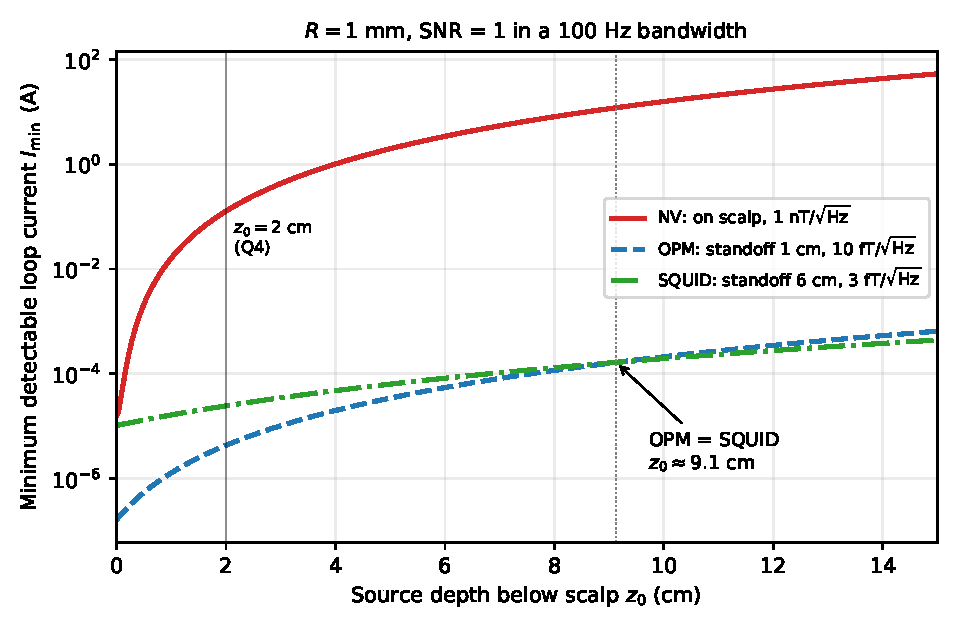
\includegraphics[width=0.86\linewidth]{q5_Imin_vs_depth.pdf}
\caption{Minimum detectable loop current (SNR $=1$, \SI{100}{\hertz} bandwidth, $R=\SI{1}{\milli\metre}$)
versus source depth $z_0$, from the exact on-axis formula. The OPM and SQUID curves cross at
$z_0\approx\SI{9.1}{\centi\metre}$; the NV curve lies above both everywhere.}
\label{fig:q5}
\end{figure}

\textbf{Limit 1: shallow source, $z_0\to0$.} The geometric factor is now dominated by the standoff,
$z\to d_i$, so proximity matters most.
\begin{itemize}[nosep]
\item NV: $z\to 0 < R$, so the dipole approximation fails; the exact formula gives the field at the
loop centre, $B=\mu_0I/2R$, so $I_{\min}=2B_{\min}R/\mu_0 = \SI{15.9}{\micro\ampere}$. The NV
improves by a factor $\approx 8000$ relative to $z_0=\SI{2}{\centi\metre}$.
\item OPM: $z\to\SI{1}{\centi\metre}$, $I_{\min} = \SI{0.16}{\micro\ampere}$.
\item SQUID: $z\to\SI{6}{\centi\metre}$, $I_{\min} = \SI{10.3}{\micro\ampere}$, only a factor
$(8/6)^3=2.4$ better than at \SI{2}{\centi\metre}, because its standoff barely changes.
\end{itemize}
The OPM remains best by a wide margin; the NV centre, even touching the source, still needs
$98.5\times$ more current than the OPM, because its noise is $10^5$ times higher. For the NV to
match the OPM at $z_0=0$ its sensitivity would have to improve to about $\SI{10}{\pico\tesla}\sqHz$.
So shallow sources (children, small animals) favour the sensor that can be placed closest
\emph{without} giving up too much sensitivity, which is the OPM's selling point.

\textbf{Limit 2: deep source, $z_0\sim\SI{10}{\centi\metre}$ and beyond.} Now $z_0\gg d_i$, so
$(z_0+d_i)^3\to z_0^3$ for every sensor: all three curves rise as $z_0^3$ and their ratios tend to the
ratios of their sensitivities,
\[
\frac{I_{\min}^{\mathrm{SQUID}}}{I_{\min}^{\mathrm{OPM}}}\;\to\;\frac{S_{\mathrm{SQUID}}}{S_{\mathrm{OPM}}}=0.3,
\qquad
\frac{I_{\min}^{\mathrm{NV}}}{I_{\min}^{\mathrm{OPM}}}\;\to\;10^{5}.
\]
Proximity no longer helps: the standoff is a small correction to a large distance, and the raw
sensitivity decides. The SQUID therefore overtakes the OPM. The crossover follows from
$S_{\mathrm{OPM}}(z_0+\SI{1}{\centi\metre})^3 = S_{\mathrm{SQUID}}(z_0+\SI{6}{\centi\metre})^3$:
\[
\frac{z_0+6}{z_0+1} = \Big(\frac{10}{3}\Big)^{1/3} = 1.494
\;\Rightarrow\;
z_0 = \frac{6-1.494}{1.494-1}\ \mathrm{cm} = \SI{9.1}{\centi\metre},
\]
which the exact formula confirms ($\SI{9.12}{\centi\metre}$, the crossing marked in
Fig.~\ref{fig:q5}). At $z_0 = \SI{10}{\centi\metre}$ the currents are \SI{0.20}{\milli\ampere}
(SQUID), \SI{0.21}{\milli\ampere} (OPM) and \SI{16}{\ampere} (NV).

\textbf{Check.} The deep-limit trend was confirmed numerically: the ratio
$I_{\min}^{\mathrm{SQUID}}/I_{\min}^{\mathrm{OPM}}$ is $0.92$, $0.47$ and $0.35$ at
$z_0 = 0.1$, $0.3$ and \SI{1}{\metre}, approaching $0.3$. The crossover depth was found
independently by scanning numerically summed Biot--Savart fields (\SI{9.12}{\centi\metre}).

\textbf{Discussion.} Moving the source from \SI{2}{\centi\metre} to \SI{10}{\centi\metre} raises the
minimum detectable current of the best sensor by a factor of about 45 (\SI{4.3}{\micro\ampere} to
\SI{0.2}{\milli\ampere}), which is why deep-brain sources are hard to see with any magnetometer.
In practice, deep-source MEG would also rely on longer averaging (smaller $\Delta f$) and on
many-channel arrays, but the ranking set by $S z^3$ remains the core trade-off.

\begin{answerbox}
Shallow ($z_0\to0$): OPM best ($\SI{0.16}{\micro\ampere}$), then SQUID ($\SI{10}{\micro\ampere}$), then NV
($\SI{16}{\micro\ampere}$). Deep ($z_0\gtrsim\SI{9.1}{\centi\metre}$): SQUID best, with
$I_{\min}^{\mathrm{SQUID}}/I_{\min}^{\mathrm{OPM}}\to0.3$; all $I_{\min}\propto z_0^3$.
\closing{proximity dominates for shallow sources, where the OPM is clearly the best sensor and even an
NV centre on the source needs about 100 times more current, while for deep sources the standoff
becomes irrelevant and the most sensitive device wins, with the SQUID overtaking the OPM beyond a depth
of about \SI{9.1}{\centi\metre} and all minimum detectable currents growing as $z_0^3$
(Fig.~\ref{fig:q5}).}
\end{answerbox}

% =====================================================================
\section{Shared information for Questions 6--11}

\begin{problembox}{Questions 6--11: atom-interferometer gravity sensor}
An atom interferometer is used as a gravity sensor to measure small changes in gravitational
acceleration. The interferometer consists of a Mach--Zehnder configuration, where a cloud of
rubidium-87 atoms at a temperature $T = 1~\mu\mathrm{K}$ is split into two parts, recombined, and
then detected. The wavelength of the atoms is $\lambda = 780$~nm, the time between interferometer
pulses is $\tau = 100$~ms and the separation between the paths in the interferometer is $d=10$~mm.
\end{problembox}

The ``wavelength of the atoms'', $\lambda = \SI{780}{\nano\metre}$, is the wavelength of the Rb D2
optical transition, i.e.\ of the laser light that drives the atoms' beam-splitter and mirror
pulses. It is used in Q7--Q8 for the light's wave vector. The atoms' own de Broglie wavelength is a
different quantity, computed in Q6.

% =====================================================================
\section{Question 6}

\begin{problembox}{Question 6 \hfill [5 marks]}
Calculate the de Broglie wavelength $(\lambda_{\mathrm{dB}})$ of the rubidium-87 atoms.
\end{problembox}

\textbf{Principle.} De Broglie: a particle of momentum $p$ has wavelength $\lambda_{\mathrm{dB}} = h/p$
(as in the Week 3 lecture). For a cloud at temperature $T$, the momenta are thermally distributed,
so the characteristic wavelength is the \emph{thermal} de Broglie wavelength,
\[
\lambda_{\mathrm{dB}} = \frac{h}{\sqrt{2\pi m k_B T}},
\]
the standard definition for a gas, which follows from the Maxwell--Boltzmann momentum distribution.

\textbf{Working.} $m = 86.909\times\SI{1.6605e-27}{\kilogram} = \SI{1.4432e-25}{\kilogram}$ and
$k_BT = \SI{1.3806e-29}{\joule}$:
\begin{align*}
\lambda_{\mathrm{dB}} &= \frac{\SI{6.6261e-34}{\joule\second}}
{\sqrt{2\pi(\SI{1.4432e-25}{\kilogram})(\SI{1.3806e-29}{\joule})}}
= \frac{\SI{6.6261e-34}{\joule\second}}{\SI{3.538e-27}{\kilogram\metre\per\second}}\\
&= \SI{1.87e-7}{\metre} \approx \SI{187}{\nano\metre}.
\end{align*}

\textbf{Check.} Units: $\si{\joule\second}/\sqrt{\si{\kilogram\joule}} = \si{\joule\second}/(\si{\kilogram\metre\per\second}) = \si{\metre}$.
The same value follows from the momentum-space partition function evaluated by numerical
quadrature. As a sanity check on the size, the rms speed is $v_{\mathrm{rms}} = \sqrt{3k_BT/m} =
\SI{1.7}{\centi\metre\per\second}$, so $h/(m v_{\mathrm{rms}}) = \SI{271}{\nano\metre}$: the same order
of magnitude, differing only by the numerical factor $\sqrt{2\pi/3}$ in the choice of
characteristic speed. Either way $\lambda_{\mathrm{dB}}$ is comparable to the optical wavelength,
which is why ultracold atoms behave as coherent matter waves.

\begin{answerbox}
$\lambda_{\mathrm{dB}} = h/\sqrt{2\pi m k_BT} \approx \SI{1.9e-7}{\metre} = \SI{187}{\nano\metre}$
\ (or \SI{271}{\nano\metre} if the rms speed is used).
\closing{the thermal de Broglie wavelength of the \SI{1}{\micro\kelvin} rubidium-87 atoms is about
\SI{190}{\nano\metre}, a quarter of the \SI{780}{\nano\metre} laser wavelength and several hundred
times the size of the atom itself (about \SI{0.5}{\nano\metre}).}
\end{answerbox}

% =====================================================================
\section{Question 7}

\begin{problembox}{Question 7 \hfill [5 marks]}
Suppose the gravitational acceleration in the absence of any perturbations is
$g_0 = 9.8~\mathrm{m}/\mathrm{s}^2$. If the interferometer is sensitive to changes in gravitational
acceleration at a level of $\Delta g = 1.0\times10^{-9}~\mathrm{m/s}^2$, calculate the corresponding
phase shift $(\Delta\varphi)$ in the interferometer.
\end{problembox}

\textbf{Principle.} In a light-pulse (Mach--Zehnder) atom interferometer the three pulses
($\pi/2$--$\pi$--$\pi/2$), separated by $\tau$, imprint the local phase of the laser light,
$k_{\mathrm{eff}}z$, onto the atoms. The phase difference read out is
$\varphi = k_{\mathrm{eff}}\,[z(0)-2z(\tau)+z(2\tau)]$. For a freely falling atom,
$z(t) = z_0+v_0t-\tfrac12 g t^2$, the terms in $z_0$ and $v_0$ cancel and
\[
\varphi = k_{\mathrm{eff}}\big[0 + g\tau^2 - 2g\tau^2\big] \;\Rightarrow\; |\varphi| = k_{\mathrm{eff}}\,g\,\tau^2 ,
\]
the acceleration term of the lecture's Eq.~(3.1). The phase is linear in $g$, so a change $\Delta g$
gives $\Delta\varphi = k_{\mathrm{eff}}\Delta g\,\tau^2$. The counter-propagating Raman beams each
transfer momentum $\hbar k$ in opposite directions, so $k_{\mathrm{eff}} = k_1+k_2 \approx 2k = 4\pi/\lambda$
(Week 3, Fig.~3.4).

\textbf{Working.}
\begin{align*}
k_{\mathrm{eff}} &= \frac{4\pi}{\SI{780e-9}{\metre}} = \SI{1.611e7}{\per\metre},\\
\Delta\varphi &= (\SI{1.611e7}{\per\metre})(\SI{1.0e-9}{\metre\per\second\squared})(\SI{0.1}{\second})^2
= \SI{1.61e-4}{\radian}.
\end{align*}
For scale, the full gravitational phase is $k_{\mathrm{eff}}g_0\tau^2 = \SI{1.58e6}{\radian}$, so
$\Delta\varphi/\varphi = \Delta g/g_0 = 10^{-10}$: the interferometer must resolve one part in
$10^{10}$ of its total phase.

\textbf{Check.} Units: $\si{\per\metre}\cdot\si{\metre\per\second\squared}\cdot\si{\second\squared}$ is
dimensionless (radians). Integrating the atom's trajectory numerically for $g_0$ and
$g_0+\Delta g$ and evaluating $k_{\mathrm{eff}}[z_1-2z_2+z_3]$ gives
$\Delta\varphi = \SI{1.61e-4}{\radian}$.

\begin{notebox}
The question also quotes a path separation $d=\SI{10}{\milli\metre}$, which the formula above does
not use. The separation is fixed by the recoil: $d = (\hbar k_{\mathrm{eff}}/m)\,\tau = \SI{1.2}{\milli\metre}$
for the stated $\lambda$ and $\tau$. Writing the phase as $\Delta\varphi = m\,\Delta g\,d\,\tau/\hbar$
(the gravitational potential difference across the two paths) gives exactly $k_{\mathrm{eff}}\Delta g\tau^2$ for
that $d$. Inserting $d=\SI{10}{\milli\metre}$ instead (as with large-momentum-transfer beam splitters,
about $8.5\hbar k_{\mathrm{eff}}$) would give $\Delta\varphi = \SI{1.37e-3}{\radian}$. The answer
above uses the stated $\lambda$ and $\tau$, which are mutually consistent.
\end{notebox}

\begin{answerbox}
$\Delta\varphi = k_{\mathrm{eff}}\,\Delta g\,\tau^2 = \dfrac{4\pi}{\lambda}\Delta g\,\tau^2 \approx \SI{1.6e-4}{\radian}$.
\closing{a change in gravitational acceleration of \SI{1.0e-9}{\metre\per\second\squared} produces a
phase shift of about \SI{1.6e-4}{\radian} (\SI{0.16}{\milli\radian}) in the interferometer, one part in
$10^{10}$ of the total gravitational phase of $\SI{1.6e6}{\radian}$.}
\end{answerbox}

% =====================================================================
\section{Question 8}

\begin{problembox}{Question 8 \hfill [5 marks]}
Evaluate the sensitivity $(S)$ of the atom interferometer as a gravity sensor, defined as the ratio
of the phase shift $(\Delta\varphi)$ to the change in gravitational acceleration $(\Delta g)$. Express
the sensitivity in units of radians per unit of gravitational acceleration
$(\mathrm{rad}/(\mathrm{m}/\mathrm{s}^{2}))$.
\end{problembox}

\textbf{Principle.} Because $\varphi = k_{\mathrm{eff}}g\tau^2$ is linear in $g$, the ratio
$\Delta\varphi/\Delta g$ is the same for any $\Delta g$ and equals the response factor
$k_{\mathrm{eff}}\tau^2$. It depends only on the laser wavelength and the pulse separation.

\textbf{Working.}
\[
S = \frac{\Delta\varphi}{\Delta g} = k_{\mathrm{eff}}\tau^2
= (\SI{1.611e7}{\per\metre})(\SI{0.1}{\second})^2
= \SI{1.61e5}{\radian\per(\metre\per\second\squared)} .
\]
Equivalently, from Q7: $\SI{1.61e-4}{\radian}/\SI{1.0e-9}{\metre\per\second\squared} = \SI{1.61e5}{}$.

\textbf{Check.} A linear fit of numerically integrated phases against $g$ gives a slope of
$\SI{1.611e5}{\radian\per(\metre\per\second\squared)}$. In gravimetry units this is
\SI{1.6}{\milli\radian} per \si{\micro Gal} ($\SI{1}{\micro Gal} = \SI{e-8}{\metre\per\second\squared}$).
Because $S\propto\tau^2$, doubling the pulse separation would quadruple it, which is why
interrogation time is the main design lever (Week 3).

\begin{answerbox}
$S = k_{\mathrm{eff}}\tau^2 = 4\pi\tau^2/\lambda \approx \SI{1.6e5}{\radian\per(\metre\per\second\squared)}$.
\closing{the atom interferometer's sensitivity as a gravity sensor is about
$\SI{1.6e5}{}$ radians per \si{\metre\per\second\squared} of acceleration change, i.e.\ every
\si{\micro Gal} of gravity change shifts the phase by about \SI{1.6}{\milli\radian}.}
\end{answerbox}

% =====================================================================
\section{Question 9}

\begin{problembox}{Question 9 \hfill [10 marks]}
Using the force of gravitation $F=G\,m_1 m_2/r^2$ between two masses $m_1$ and $m_2$ at a distance
$r$ between them, what is the change of gravitational acceleration an atom experiences due to:
the presence of the moon pulling into or against the direction of the Earth's gravitational
acceleration (tidal effects)? The moon is on average about $385{,}000$~km from the Earth and its mass
is about $7.3\times 10^{22}$~kg.
\end{problembox}

\textbf{Principle.} Dividing Newton's force by the atom's mass gives the acceleration due to a mass
$M$ at distance $r$: $a = GM/r^2$. The Moon's direct pull at the Earth's distance is
\[
a_{\mathrm{Moon}} = \frac{GM}{r^2} = \frac{(\SI{6.674e-11}{})(\SI{7.3e22}{\kilogram})}{(\SI{3.85e8}{\metre})^2}
= \SI{3.3e-5}{\metre\per\second\squared}.
\]
However, this is \emph{not} what a gravimeter on Earth measures. The Moon accelerates the whole Earth,
including the instrument, by almost exactly this amount; the Earth is in free fall towards the Moon.
The sensor measures only the \emph{difference} between the Moon's pull at its location and at the
Earth's centre. This difference is the tidal acceleration, which the question asks for. For a sensor
on the Earth--Moon line, a distance $R_E$ nearer the Moon,
\[
\Delta g = \frac{GM}{(r-R_E)^2}-\frac{GM}{r^2} \approx \frac{2GMR_E}{r^3}\qquad(R_E\ll r),
\]
by the expansion $(1-x)^{-2}\approx 1+2x$ with $x = R_E/r = 0.017$.

\textbf{Working.}
\[
\Delta g = \frac{2(\SI{6.674e-11}{})(\SI{7.3e22}{\kilogram})(\SI{6.371e6}{\metre})}{(\SI{3.85e8}{\metre})^3}
= \frac{\SI{6.21e19}{}}{\SI{5.71e25}{}}\ \si{\metre\per\second\squared}
= \SI{1.1e-6}{\metre\per\second\squared}.
\]
\emph{Direction.} With the Moon overhead (or directly underfoot), the tidal acceleration points away
from the Earth's centre, against $g$, so $g$ is reduced by $\approx\SI{1.1e-6}{\metre\per\second\squared}$.
With the Moon on the horizon, it points towards the Earth's centre, along $g$, adding
$GMR_E/r^3 = \SI{0.54e-6}{\metre\per\second\squared}$. As the Earth rotates, $g$ therefore swings by about
\SI{1.6e-6}{\metre\per\second\squared} peak-to-peak, twice a day.

\textbf{Check.} Evaluating the exact difference without approximation gives
\SI{1.12e-6}{\metre\per\second\squared} on the near side and \SI{1.06e-6}{\metre\per\second\squared}
on the far side; their mean is \SI{1.09e-6}{}, matching $2GMR_E/r^3$. The magnitude agrees with
measured Earth tides (of order \SI{100}{\micro Gal}).

\begin{answerbox}
Tidal change $\Delta g \approx 2GMR_E/r^3 \approx \SI{1.1e-6}{\metre\per\second\squared}$
(about \SI{110}{\micro Gal}, $\approx 1100\,\Delta g_{\min}$); direct pull $GM/r^2 = \SI{3.3e-5}{\metre\per\second\squared}$
is not observable because the Earth falls with it.
\closing{the Moon changes the gravitational acceleration experienced by the atoms by about
\SI{1.1e-6}{\metre\per\second\squared}, against $g$ when it is overhead and along $g$ (by half as much)
when it is on the horizon. This is roughly a thousand times the interferometer's
\SI{1e-9}{\metre\per\second\squared} resolution, so tides must be modelled and subtracted from every
gravity measurement.}
\end{answerbox}

% =====================================================================
\section{Question 10}

\begin{problembox}{Question 10 \hfill [10 marks]}
Using the force of gravitation $F=G\,m_1 m_2/r^2$, what is the change of gravitational acceleration an
atom experiences due to: the presence or absence of a person $(70$~kg$)$ at a distance of $1$~m. How
far away does the person have to be to create a similar effect to that of the moon? How far away can
they be and still be detected by the interferometer?
\end{problembox}

\textbf{Principle.} The person is treated as a point mass $m_p = \SI{70}{\kilogram}$. Unlike the
Moon, the person does not accelerate the instrument, so the full $Gm_p/r^2$ is the change the atoms
experience, provided the person lies along the sensitive (vertical) axis. Setting
$Gm_p/r^2$ equal to a target $\Delta g$ and inverting gives $r = \sqrt{Gm_p/\Delta g}$.

\textbf{Working.}
\begin{enumerate}[label=(\alph*), nosep, leftmargin=*]
\item At $r = \SI{1}{\metre}$:
$\displaystyle \Delta g = \frac{(\SI{6.674e-11}{})(\SI{70}{\kilogram})}{(\SI{1}{\metre})^2}
= \SI{4.7e-9}{\metre\per\second\squared}$, about $4.7\,\Delta g_{\min}$, so detectable.
\item Matching the Moon's tidal effect, $\Delta g = \SI{1.09e-6}{\metre\per\second\squared}$ (Q9):\\
$\displaystyle r = \sqrt{\frac{\SI{4.672e-9}{}}{\SI{1.09e-6}{}}}\ \si{\metre} = \SI{0.066}{\metre}\approx\SI{6.6}{\centi\metre}.$
\item Detection limit, $\Delta g_{\min} = \SI{1.0e-9}{\metre\per\second\squared}$:\\
$\displaystyle r_{\max} = \sqrt{\frac{\SI{4.672e-9}{}}{\SI{1.0e-9}{}}}\ \si{\metre} = \SI{2.2}{\metre}.$
\end{enumerate}

\textbf{Check.} Substituting back: $Gm_p/(\SI{0.0655}{\metre})^2 = \SI{1.09e-6}{}$ and
$Gm_p/(\SI{2.16}{\metre})^2 = \SI{1.00e-9}{\metre\per\second\squared}$. Ratios agree with
$\Delta g\propto r^{-2}$: going from \SI{1}{\metre} to \SI{2.16}{\metre} reduces the signal by
$2.16^2 = 4.7$, exactly the margin found in (a).

\textbf{Interpretation.} A distance of \SI{6.6}{\centi\metre} from a person's centre of mass is
inside their body: the point-mass model fails, and no person can mimic the lunar tide. The practical
lesson is the reverse. An operator standing within about \SI{2}{\metre} of the sensor perturbs the
reading by more than its resolution, so people must keep away during measurements. A person standing
\emph{beside} the instrument pulls mostly horizontally, so a vertical gravimeter sees only the vertical
component; the values above are upper bounds for the vertical axis.

\begin{notebox}
If the Moon's direct pull $GM/r^2 = \SI{3.3e-5}{\metre\per\second\squared}$ were used as the
comparison instead of the tidal value, the distance in (b) would be \SI{1.2}{\centi\metre}; the
conclusion that it is physically unreachable is unchanged.
\end{notebox}

\begin{answerbox}
(a) $\Delta g = \SI{4.7e-9}{\metre\per\second\squared}$ at \SI{1}{\metre};
(b) $r\approx\SI{6.6}{\centi\metre}$ to match the lunar tide;
(c) detectable out to $r_{\max}\approx\SI{2.2}{\metre}$.
\closing{a \SI{70}{\kilogram} person \SI{1}{\metre} away changes the atoms' gravitational acceleration
by about \SI{4.7e-9}{\metre\per\second\squared}, which the interferometer can detect out to about
\SI{2.2}{\metre}, whereas matching the Moon's tidal effect would require the person's centre of mass
to be only \SI{6.6}{\centi\metre} from the atoms, which is physically impossible.}
\end{answerbox}

% =====================================================================
\section{Question 11}

\begin{problembox}{Question 11 \hfill [15 marks]}
Using the force of gravitation $F=G\,m_1 m_2/r^2$, what is the change of gravitational acceleration an
atom experiences due to: a (spherical) void in the soil (for example, a tunnel, a sinkhole or a gas
reservoir) of a diameter of $1$~m at a distance of $3$~m? Assume the void to have zero mass density
and the surrounding soil the Earth's average density of $\rho=5.5~\mathrm{g}/\mathrm{cm}^3$. Given the
minimal detectable $\Delta g$, what is the maximal depth of the void as a function of its diameter that
is still detectable. Plot the graph of this function.
\end{problembox}

\textbf{Principle.} \emph{Superposition.} Soil containing a void is equivalent to uniform soil plus a
sphere of \emph{negative} density $-\rho$ filling the void. The uniform soil gives the normal $g_0$, so
the anomaly is the attraction of the ``missing mass''
\[
\Delta m = \rho\,\frac{4}{3}\pi\Big(\frac D2\Big)^3 = \frac{\pi}{6}\rho D^3 ,
\]
acting \emph{away} from the void. By Newton's shell theorem, a uniform sphere attracts an outside
point as if all its mass were at its centre, so the point-mass formula is exact for a spherical void,
with $r$ measured to the void's centre. Measured directly above the void, the anomaly is vertical:
\[
\Delta g = -\frac{G\,\Delta m}{r^2} = -\frac{\pi G\rho D^3}{6\,r^2}.
\]

\textbf{Working: the example.} $\rho = \SI{5500}{\kilogram\per\metre\cubed}$, $D=\SI{1}{\metre}$,
$r=\SI{3}{\metre}$:
\begin{align*}
\Delta m &= \tfrac{\pi}{6}(\SI{5500}{\kilogram\per\metre\cubed})(\SI{1}{\metre})^3 = \SI{2880}{\kilogram},\\
\Delta g &= -\frac{(\SI{6.674e-11}{})(\SI{2880}{\kilogram})}{(\SI{3}{\metre})^2}
= \SI{-2.1e-8}{\metre\per\second\squared}.
\end{align*}
Gravity is reduced by \SI{2.1e-8}{\metre\per\second\squared} (\SI{2.1}{\micro Gal}), about 21 times
the interferometer's resolution, so this void is readily detectable.

\textbf{Working: maximum detectable depth.} The void is detectable while
$|\Delta g|\ge\Delta g_{\min}$, with $\Delta g_{\min} = \SI{1.0e-9}{\metre\per\second\squared}$ (Q7).
Setting equality and solving for the depth $z$ of the void's centre below the sensor:
\[
\frac{\pi G\rho D^3}{6z_{\max}^2} = \Delta g_{\min}
\quad\Longrightarrow\quad
z_{\max}(D) = \sqrt{\frac{\pi G\rho}{6\,\Delta g_{\min}}}\;D^{3/2}.
\]
Numerically,
$\sqrt{\pi(\SI{6.674e-11}{})(\SI{5500}{})/(6\times\SI{1e-9}{})} = \SI{13.9}{\metre^{-1/2}}$, so
\[
z_{\max}(D) \approx 13.9\,D^{3/2}\quad(\text{both in metres}).
\]
Examples: $D = \SI{0.5}{\metre}\to\SI{4.9}{\metre}$; $D=\SI{1}{\metre}\to\SI{13.9}{\metre}$;
$D=\SI{2}{\metre}\to\SI{39}{\metre}$; $D=\SI{5}{\metre}\to\SI{155}{\metre}$. The result is physically
meaningful only while $z_{\max} > D/2$ (the void does not reach the sensor), which holds for all
$D > \SI{1.3}{\milli\metre}$.

\begin{figure}[H]
\centering
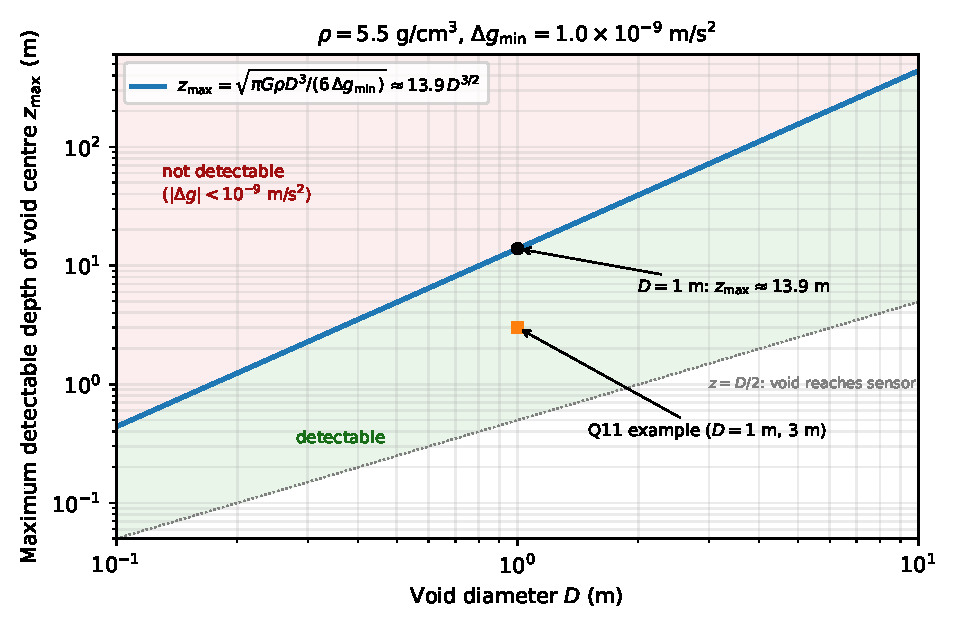
\includegraphics[width=0.86\linewidth]{q11_rmax_vs_diameter.pdf}
\caption{Maximum detectable depth of a spherical void's centre as a function of its diameter
(log--log axes, slope $3/2$). Voids below the line are detectable; the orange square is the Q11
example ($D=\SI{1}{\metre}$ at \SI{3}{\metre}).}
\label{fig:q11}
\end{figure}

\textbf{Check.} Units:
$\sqrt{(\si{\metre\cubed\per\kilogram\per\second\squared})(\si{\kilogram\per\metre\cubed})/(\si{\metre\per\second\squared})}\,\si{\metre}^{3/2}
= \si{\metre}^{-1/2}\,\si{\metre}^{3/2} = \si{\metre}$. Without using the shell theorem, a direct 3D
numerical integration of the attraction of a uniform \SI{1}{\metre} sphere gives
$|\Delta g| = \SI{2.136e-8}{\metre\per\second\squared}$ at \SI{3}{\metre}, and root-finding the
integral gives $z_{\max} = \SI{13.86}{\metre}$ for $D=\SI{1}{\metre}$ and \SI{39.21}{\metre} for
$D=\SI{2}{\metre}$, a ratio of $2^{3/2}$ as the formula predicts.

\textbf{Interpretation.} The steep $D^{3/2}$ law reflects the competition between volume ($D^3$) and
inverse-square distance ($z^{-2}$): doubling a void's diameter lets it be found at $2.8$ times the depth.
This is the basis for using quantum gravimeters to find tunnels, sinkholes and mineshafts (Week 3).
Real surveys also map $\Delta g$ along a line, since the anomaly's width (comparable to its depth) helps fix $z$,
and usually use gradiometers to cancel common vibration noise.

\begin{notebox}
The ``distance of \SI{3}{\metre}'' is taken to the void's centre. If it meant the nearest edge, $r$
would be \SI{3.5}{\metre} and $\Delta g = \SI{-1.6e-8}{\metre\per\second\squared}$, still detectable.
Q11's shared text names the pulse time $T_{\mathrm{pulse}}$ rather than $\tau$; this does not affect
the answer, which depends only on the stated $\Delta g_{\min}$.
\end{notebox}

\begin{answerbox}
$\Delta g = -\dfrac{\pi G\rho D^3}{6r^2} \approx \SI{-2.1e-8}{\metre\per\second\squared}$ for
$D=\SI{1}{\metre}$ at \SI{3}{\metre}; \quad
$z_{\max}(D) = \sqrt{\dfrac{\pi G\rho}{6\Delta g_{\min}}}\,D^{3/2} \approx 13.9\,D^{3/2}$~m
(Fig.~\ref{fig:q11}).
\closing{the \SI{1}{\metre} void \SI{3}{\metre} away reduces the atoms' gravitational acceleration by
about \SI{2.1e-8}{\metre\per\second\squared}, some 21 times the detection limit, and a spherical void
of diameter $D$ remains detectable down to a centre depth of about $13.9\,D^{3/2}$ metres, which is
\SI{14}{\metre} for a \SI{1}{\metre} void.}
\end{answerbox}

% =====================================================================
\section{Summary of results}

\begin{center}
\footnotesize
\begin{tabular}{clll}
\toprule
Q & Quantity & Result & Key relation\\
\midrule
1 & SNR of OPM & $1.26$ (\SI{2}{\decibel}) & $B_{\mathrm{sig}}/(S\sqrt{\Delta f})$\\
2 & Far-field scaling & $B\approx\mu_0R^2I/2z^3\propto z^{-3}$ & binomial expansion, $z\gg R$\\
3 & Best SNR at $z_0=\SI{2}{\centi\metre}$ & OPM ($5.7\times$ SQUID) & $\mathrm{SNR}\propto 1/Sz^3$\\
4 & $I_{\min}$ NV / OPM / SQUID & \SI{0.13}{\ampere} / \SI{4.3}{\micro\ampere} / \SI{24}{\micro\ampere} & $B(z)=S\sqrt{\Delta f}$\\
5 & Depth dependence & OPM best shallow; SQUID beyond \SI{9.1}{\centi\metre} & Fig.~\ref{fig:q5}\\
6 & $\lambda_{\mathrm{dB}}$ & \SI{187}{\nano\metre} & $h/\sqrt{2\pi mk_BT}$\\
7 & $\Delta\varphi$ & \SI{1.6e-4}{\radian} & $k_{\mathrm{eff}}\Delta g\tau^2$\\
8 & Sensitivity $S$ & \SI{1.6e5}{\radian\per(\metre\per\second\squared)} & $k_{\mathrm{eff}}\tau^2$\\
9 & Lunar tide & \SI{1.1e-6}{\metre\per\second\squared} & $2GMR_E/r^3$\\
10 & Person: 1 m / Moon / limit & \SI{4.7e-9}{\metre\per\second\squared} / \SI{6.6}{\centi\metre} / \SI{2.2}{\metre} & $Gm/r^2$\\
11 & Void; max depth & \SI{-2.1e-8}{\metre\per\second\squared}; $13.9\,D^{3/2}$ m & shell theorem, Fig.~\ref{fig:q11}\\
\bottomrule
\end{tabular}
\end{center}

\closing{all eleven questions are answered above, with every numerical result checked independently
by simulation, numerical integration or direct field summation.}

\end{document}
